\documentclass{beamer}
\title{1G/2G Europe}
\subtitle{}
\author{Malte Behrendt, Lucas Dohmen, Michael Hackstein, Nicolas Inden}
\institute{Development of IT Standards}
\date{\today}
 
\usetheme{DS}

\usepackage[english]{babel}
\usepackage[utf8]{inputenc}
\usepackage{epsf}
\usepackage{rotating}
\usepackage{ifthen}
\usepackage{graphicx}
\usepackage{amsmath}
\usepackage{amssymb}
\usepackage{alltt}
\usepackage{scalefnt}
\usepackage{epsfig}
\usepackage{psfrag}
\usepackage{enumerate}
\usepackage{xmpmulti}
\usepackage{subfigure}
\usepackage{chronology}

\begin{document}

% do the title page
\setbeamertemplate{frametitle}[empty]
\setbeamertemplate{footline}[empty]


%use this if you don't adjust the title-background image
\setbeamertemplate{background}{

\includegraphics[width=\paperwidth,height=\paperheight]{pictures/title-background-empty.pdf}}
\frame{\titlepage} 

%use this if you adjust the title-background image to display the correct stuff
%this is a dirty hack. :-(
%\setbeamertemplate{background}{
%
\includegraphics[width=\paperwidth,height=\paperheight]{pictures/title-background.pdf}}
%\frame{}



\setbeamertemplate{frametitle}[dsgroup]
\setbeamertemplate{footline}[dsgroup]
\setcounter{page}{1} 
\setbeamertemplate{background}{}

% content goes here
\section{Introduction}
% Overview or introduction of 1G?
\section{1G}
\begin{frame}
  \frametitle{Nordic Mobile Telephone (NMT)}
  
  \begin{center}
    % TODO: Please add the picture to the repository!
    % 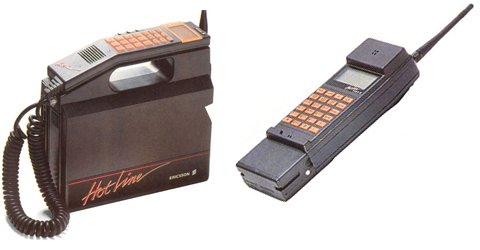
\includegraphics[width=0.55\columnwidth]{./pictures/ericsson-hotline-nmt900.jpg}
  \end{center}
\end{frame}

\begin{frame}
  \frametitle{Motivation and features}
  
    \begin{itemize}
     \item Motivation
     \begin{itemize}
      \item Overcrowding of manual mobile networks
      \item Neighboring countries used incompatible technologies
     \end{itemize}
    \end{itemize}
    
    \begin{center}
     $\Rightarrow$ Addressed by national telephone operators from\\Denmark, Finnland, Norway and Sweden
    \end{center}
    
    \begin{itemize}
     \item Results
      \begin{itemize}
	\item Same services as landline
        \item Automatized handover between calls
        \item National and international roaming
      \end{itemize}
    \end{itemize}
\end{frame}

\begin{frame}
  \frametitle{Negotiation and diffusion}
  
  \begin{chrono}[10]{1969}{1986}{3ex}{\textwidth}
    \event{1969}{Vision of a standardized system}
    \event{1970}{First meeting of operator representatives}
    %\event{1971}{System specification}
    \event[1981]{1982}{NMT-450 release (on time)}
    \event{1985}{Largest cellular phone system world-wide}
    \event{1986}{NMT-900 release}
  \end{chrono}
  
  \begin{center}
     $\Rightarrow$ NMT became a \textbf{global} standard
    \end{center}
\end{frame}

\begin{frame}
  \frametitle{Success factors}
  
  % umformulieren!
  \begin{itemize}
   \item Market orientation 
   \item Small working groups
   \item Negotiation restricted to interface specifications
   \item Intense relationship to manufacturers but neutral treatment
   \item Economies of scale due to open specification and lack of IPRs/no license fees 
   \item No/little government/national institutions involvement
  \end{itemize}
\end{frame}

%england
\frame{
	\frametitle{1G: Germany}
	
	\begin{columns}
		\begin{column}{0.4\textwidth}
			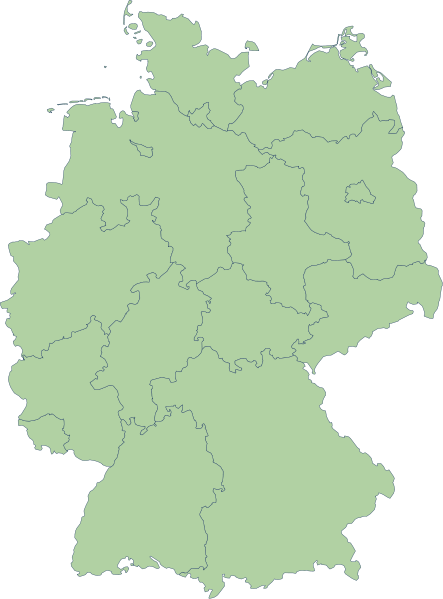
\includegraphics[width=\textwidth]{pictures/deutschland}
		\end{column}
	
		\hfill
	
		\begin{column}{0.59\textwidth}
			\begin{center}
				
\includegraphics[width=0.5\textwidth]{pictures/bundespost}
			\end{center}
			\begin{itemize}
				\item Responsible provider: Deutsche Bundespost
				\item Monopoly of DBP as only provider
				\item Network was finished in 1985, years after Japan, US and NMT
				\item Since 1989: DBP Telekom
			\end{itemize}
			
\includegraphics[width=\textwidth]{pictures/cnetz}
		\end{column}
	\end{columns}
}

\frame{
	\frametitle{1G: Germany}
	
	\begin{columns}
		\begin{column}{0.7\textwidth}
			
\includegraphics[width=0.5\textwidth]{pictures/siemens}
	
			\textbf{Development of the} 
\includegraphics[height=0.3cm]{pictures/cnetz_orig} \textbf{-Net}
	
			\begin{itemize}
				\item Innovation process started in 1979
				\item Siemens was assigned to develop the technology
				\item Intention of creating a superior technology
				\item Start was postponed in favor of advanced technology
				\item Result: The German 1G approach was late
			\end{itemize}
			
		\end{column}
		\hfill
		\begin{column}{0.29\textwidth}
			\begin{figure}[t]
				
\includegraphics[width=\textwidth]{pictures/antenne}
			\end{figure}
		\end{column}
	\end{columns}
}

\frame{
	\frametitle{1G: Germany}
	
	\textbf{Failure factors of the C-Net}
	
	\begin{itemize}
		\item \textbf{It was proprietary, a closed system}
			\begin{itemize}
				\item The closed system caused a monopoly for infrastructure and handsets
			\end{itemize}
		\item \textbf{It was expensive}
			\begin{itemize}
				\item Lack of competition in Germany
				\item This also prevented prices from falling
				\item If amount of users reaches capacity limits, prices were raised
				\item In contrast: NMT fixed their technology to cope the demand
			\end{itemize}
		\item \textbf{Only few attracted users}
			\begin{itemize}
				\item Missing positive externalities
			\end{itemize}
		\item \textbf{The lack of leadership}
			 \begin{itemize}
				 \item Neither government nor companies formed a committee
			 \end{itemize}
	\end{itemize}
}
\section{2G}
\begin{frame}{GSM History}
  \begin{description}
    \item[1982] CEPT started GSM %CEPT was only open for operators
    \item[Until Feb. 1987] Different technologies and proposals presented.
    \begin{itemize}
      \item No \emph{general architecture patenting} or \emph{non-disclosure patenting strategy}
    \end{itemize}
    \item[1988] CEPT was replaced by ETSI %Also open for manufacturers and privately owned operators
    \begin{itemize}
      \item Members have to notify essential IPRs (140 distinct IPRs in 1998)
      \item Motorola: \emph{license without general declaration}
      \item Others: \emph{gentleman's agreement}
    \end{itemize}
    \item[1990-1993] Siemens, Alcatel, Nokia and Ericsson enter cross-license agreement with Motorola
    \item[1993] \emph{licensing-by-default} (abandoned due to complaints)
    \item[Next Policy] Members inform ETSI about IPRs, ETSI negotiates licence conditions
    \item[1994] GSM became big success
  \end{description}
\end{frame}

\section{Conclusion}

\bibliographystyle{plain}

\end{document}
